% !TEX TS-program = pdflatex
% !TEX encoding = UTF-8 Unicode

\documentclass[a4paper, titlepage=false, parskip=full-, 10pt]{scrartcl}

\usepackage[utf8]{inputenc}
\usepackage[T1]{fontenc}
\usepackage[english, ngerman]{babel}
\usepackage{babelbib}
\usepackage{hyperref}
\usepackage{listings}
\usepackage{framed}
\usepackage{color}
\usepackage{graphicx}
\usepackage[normalem]{ulem}
\usepackage{cancel}
\usepackage{amsmath}
\usepackage{amssymb}
\usepackage{amsthm}
\usepackage{algorithm}
\usepackage{algorithmic}
\usepackage{geometry}
\usepackage{subfigure}
\geometry{a4paper, top=20mm, left=35mm, right=25mm, bottom=40mm}

\newcounter{tasknbr}
\setcounter{tasknbr}{1}
\newenvironment{task}[1]{{\bf Aufgabe \arabic {tasknbr}\stepcounter{tasknbr}} (#1):\begin{enumerate}}{\end{enumerate}}
\newcommand{\subtask}[1]{\item[#1)]}

% Listings -----------------------------------------------------------------------------
\definecolor{red}{rgb}{.8,.1,.2}
\definecolor{blue}{rgb}{.2,.3,.7}
\definecolor{lightyellow}{rgb}{1.,1.,.97}
\definecolor{gray}{rgb}{.7,.7,.7}
\definecolor{darkgreen}{rgb}{0,.5,.1}
\definecolor{darkyellow}{rgb}{1.,.7,.3}
\lstloadlanguages{C++,[Objective]C,Java}
\lstset{
escapeinside={§§}{§§},
basicstyle=\ttfamily\footnotesize\mdseries,
columns=fullflexible, % typewriter font look better with fullflex
keywordstyle=\bfseries\color{blue},
% identifierstyle=\bfseries,
commentstyle=\color{darkgreen},      
stringstyle=\color{red},
numbers=left,
numberstyle=\ttfamily\scriptsize\color{gray},
% stepnumber=5,
% numberfirstline=true,
breaklines=true,
% prebreak=\\,
showstringspaces=false,
tabsize=4,
captionpos=b,
% framexrightmargin=-.2\textwidth,
float=htb,
frame=tb,
frameshape={RYR}{y}{y}{RYR},
rulecolor=\color{black},
xleftmargin=15pt,
xrightmargin=4pt,
aboveskip=\bigskipamount,
belowskip=\bigskipamount,
backgroundcolor=\color{lightyellow},
extendedchars=true,
belowcaptionskip=15pt}

%% Enter current values here: %%
\newcommand{\lecture}{Algorithmische Geometrie SS15}
\newcommand{\tutor}{}
\newcommand{\assignmentnbr}{5}
\newcommand{\students}{Julius Auer, Alexa Schlegel}
%%-------------------------------------%%

\begin{document}  
{\small \textsl{\lecture \hfill \tutor}}
\hrule
\begin{center}
\textbf{Übungsblatt \assignmentnbr}\\
[\bigskipamount]
{\small \students}
\end{center}
\hrule

\begin{task}{Suchen in ebenen Unterteilungen}
\item[]

Eine ebene Unterteilung ist eine Partition von \mathbb{R}^2 in durch Strecken und Strahlen begrenzte Gebiete (Einbettung eines planaren Graphen $G$)\\



* einfache Datenstruktur beschreiben zum Suchen mit Anfragezeit $O(\log n)$\\
* Vorverarbeitungszeit\\
* Speicherplatz für Datensturktur
\end{task}

\begin{task}{$L_1$-Voronoi-Diagramme}
\item[]
Für zwei Punkte $p=(p_x, p_y)$ und $q=(q_x, q_y)$ ist die $L_1$-Metrik wie folgt definiert:\\ $d_1=\left|p_x-q_x\right| + \left|p_y-q_y\right|$

Es lassen sich drei Fälle unterscheiden, je nach dem in welchem Verhältnis die Differenz der $x$ bzw. $y$ Werte der Punkte $p$ und $q$ zueinander stehen.

Fall {\large\textcircled{\small{1}}}: $\left|p_x-q_x\right| < \left|p_y-q_y\right|$\\
Fall {\large\textcircled{\small{2}}}: $\left|p_x-q_x\right| > \left|p_y-q_y\right|$\\
Fall {\large\textcircled{\small{3}}}: $\left|p_x-q_x\right| = \left|p_y-q_y\right|$\\

\begin{figure}[h]
\begin{center}
\subfigure{
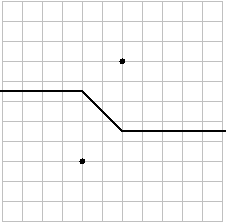
\includegraphics[width=3cm]{capture1}
}
\subfigure{
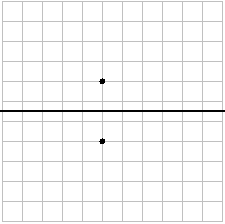
\includegraphics[width=3cm]{capture2}
}
\subfigure{
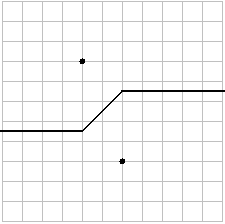
\includegraphics[width=3cm]{capture3}
}
\end{center}
\caption{Fall 1: Bisektor verläuft in Richtung der $x$-Achse, horizontal}
\end{figure}

\begin{figure}[h]
\begin{center}
\subfigure{
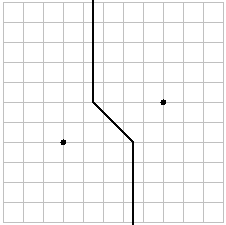
\includegraphics[width=3cm]{capture4}
}
\subfigure{
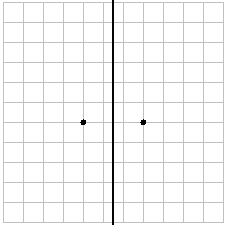
\includegraphics[width=3cm]{capture5}
}
\subfigure{
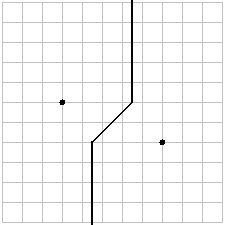
\includegraphics[width=3cm]{capture6}
}
\end{center}
\caption{Fall 2: Bisektor verläuft in Richtung der $y$-Achse, vertikal}
\end{figure}

\begin{figure}[h]
\begin{center}
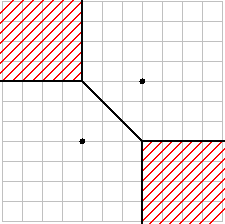
\includegraphics[width=4cm]{capture7}
\end{center}
\caption{Fall 3: Bisektor besteht aus zwei unbeschränkten Bereichen und einer Strecke.}
\end{figure}
\end{task}

\begin{task}{Suche in ebenen Unterteilungen - Verallgemeinerung}
\item[]


* Erweiterung von LDS\\
* Algorithmen zur Suche und Konstruktion anpassen\\
* alle Unterteilungen den Ebene sollen unterstützt werden (mehrere unbeschränkte Facetten)\\
* Einzelheiten der Algorithmen beschreiben\\
*Vorverarbeitungszeit, Speicherbedarf, Anfragezeit, Anhängig von Anzahl der Knoten\\ 

\end{task}
\end{document}